\documentclass[final]{beamer}

% ====================
% Packages
% ====================

\usepackage[T1]{fontenc}
\usepackage[utf8]{luainputenc}
\usepackage[style=ieee]{biblatex}
\usepackage[sfdefault]{roboto}

\newif\ifazerosize
% \azerosizetrue
\ifazerosize
% A0
\usepackage[size=custom, width=84.1, height=118.9, scale=1.45]{beamerposter}
\else
% 36 in by 48 in
\usepackage[size=custom, width=91.44, height=121.92, scale=1.45]{beamerposter}
\fi


\usetheme{gemini}
\usecolortheme{gemini}
\usepackage{graphicx}

\usepackage{tikz}
\usepackage{pgfplots}
\pgfplotsset{compat=1.14}
\usepackage{anyfontsize}

\usepackage{fontawesome5}

\usepackage{lipsum}

\usepackage{tabularx}
\usepackage{booktabs}

\usepackage{siunitx}
\sisetup{detect-all}

\usepackage{amsfonts}
\usepackage{amsmath}
\usepackage{amssymb}

\hyphenpenalty=10000

\addbibresource{references.bib}

% ====================
% Lengths
% ====================

% If you have N columns, choose \sepwidth and \colwidth such that
% (N+1)*\sepwidth + N*\colwidth = \paperwidth

\newlength{\sepwidth}
\newlength{\colwidth}
\setlength{\sepwidth}{0.025\paperwidth}
\setlength{\colwidth}{0.4625\paperwidth}

\newcommand{\separatorcolumn}{\begin{column}{\sepwidth}\end{column}}

% ====================
% Title
% ====================

\title{Genhack 3 - Hackathon For Generative Modelling}

\author{Clément Combier, Ludovic Bossard, El Houssaine Chahboun and Gaoyuan Zhou}

\institute[shortinst]{Deneter's Vision, École Polytechnique and PNB Paribas}

% ====================
% Footer (optional)
% ====================

\footercontent{
    \href{https://github.com/Ttiki/GenHack3-2024-Poster}{\faGithub\hspace{0.5ex} Ttiki/GenHack3-2024-Poster}
    \hfill
    \href{https://www.polytechnique.edu/en/genhack-3-hackathon-generative-modelling}{\faLink\hspace{0.5ex} www.polytechnique.edu}
    \hfill
    \href{mailto:clement.combier@etud.univ-pau.fr}{\faEnvelope\hspace{0.5ex} clement.combier@etud.univ-pau.fr}}
% (can be left out to remove footer)

% ====================
% Logo (optional)
% ====================

% use this to include logos on the left and/or right side of the header:
% Left: institution
 \logoright{
\includegraphics[height=5cm]{logos/Logo-Ecole-polytechnique-horizontal-jpeg-HD.jpg}}
% Right: funding agencies and other affilations 
%\logoright{\includegraphics[height=7cm]{logos/NSF.eps}}
% ====================
% Body
% ====================

\begin{document}

\begin{frame}[t]
\begin{columns}[t]
\separatorcolumn

\begin{column}{\colwidth}
    \begin{block}{Abstract}
        In the face of global warming and its impact on agriculture, GenHack 3 emerges as a pivotal event. This hackathon, focusing on generative modelling, seeks to address the urgent need for resilient solutions in the context of climate change. Join us in exploring innovative ways to augment datasets and simulate future maize yields, making a significant contribution to sustainable agriculture.
    \end{block}

    \begin{block}{Context}
        Human activities, notably greenhouse gas emissions, have unequivocally contributed to a 1.1°C rise in the global surface temperature \cite{Calvin2023}. This has profound effects on agriculture, manifesting in early heatwaves, altered rainfall patterns, and late frosts. As farmers bear witness to these impacts, GenHack 3 aims to define resilient solutions and develop new tools crucial for the future of agriculture in the face of climate change. 
    \end{block}

    \begin{block}{Objectives}
        GenHack 3 presents a data challenge employing generative models to understand the evolution of maize yield amid climate change. The primary objective is to augment and enrich the dataset with new data, paving the way for simulating potential future yield values. Join us in this intellectual endeavor to contribute to solutions that account for changes in temperature and rainfall, ensuring a sustainable future for agriculture.
    \end{block}

    \begin{block}{Timeline}
        \begin{figure}
            \centering
            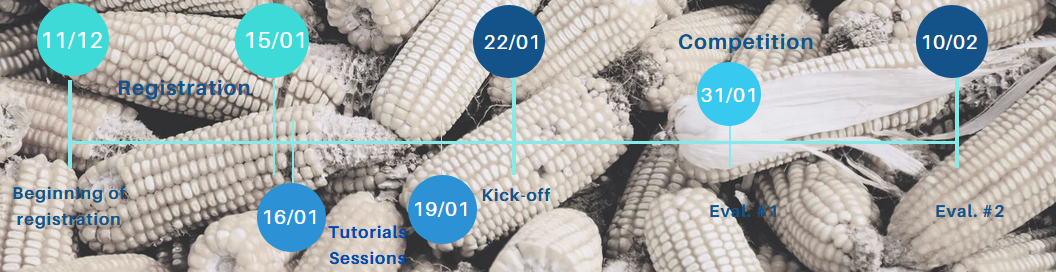
\includegraphics[width=\columnwidth]{figures/2024-Timeline_2.png}
            \caption{Official timeline of GenHack 3 2024 \cite{polytechniqueGenhackHackathon}}
            \label{fig:ftcat}
        \end{figure}
        Key Dates:
        \begin{itemize}
            \item Registration: Closed on January 15, 2024.
            \item Tutorials \& Team Building: January 16-19, 2024.
            \item Kick-off: January 22, 2024.
            \item Competition: January 22 - February 10, 2024.
            \item Evaluation #1: February 3, 2024.
            \item Evaluation #2: February 10, 2024.
        \end{itemize}
    \end{block}

    \begin{block}{Registration \& Competition Rules}
        \textbf{Registration Details:}
        \begin{itemize}
            \itexm Registrations Closed on January 15, 2024.
        \end{itemize}
        
        \textbf{Competition Rules:}
        \begin{itemize}
            \item Teams: 3 to 5 students.
            \item Code: Python only.
            \item Collaboration encouraged.
            \item Winning team members must prove student status.
        \end{itemize}
    
    \end{block}
\end{column}

\separatorcolumn

\begin{column}{\colwidth}
    \begin{column}{\colwidth}
    \begin{block}{Résumé}
        Face au réchauffement climatique et à son impact sur l'agriculture, GenHack 3 émerge comme un événement essentiel. Ce hackathon, axé sur la modélisation générative, vise à répondre au besoin urgent de solutions résilientes dans le contexte du changement climatique. Rejoignez-nous pour explorer des moyens innovants d'augmenter les ensembles de données et de simuler les rendements futurs du maïs, contribuant ainsi de manière significative à une agriculture durable.
    \end{block}

    \begin{block}{Contexte}
        Les activités humaines, notamment les émissions de gaz à effet de serre, ont contribué de manière indiscutable à une augmentation de 1,1 °C de la température de surface mondiale \cite{Calvin2023}. Cela a des effets profonds sur l'agriculture, se manifestant par des vagues de chaleur précoces, des changements de régime des précipitations et des gelées tardives. En tant que témoins de ces impacts, GenHack 3 vise à définir des solutions résilientes et à développer de nouveaux outils cruciaux pour l'avenir de l'agriculture face au changement climatique.
    \end{block}

    \begin{block}{Objectifs}
        GenHack 3 présente un défi de données utilisant des modèles génératifs pour comprendre l'évolution du rendement du maïs face au changement climatique. L'objectif principal est d'augmenter et d'enrichir l'ensemble de données avec de nouvelles données, ouvrant la voie à la simulation de valeurs potentielles de rendement futur. Rejoignez-nous dans cette démarche intellectuelle pour contribuer à des solutions qui tiennent compte des changements de température et de précipitations, assurant un avenir durable pour l'agriculture.
    \end{block}

    \begin{block}{Chronologie}
        \begin{figure}
            \centering
            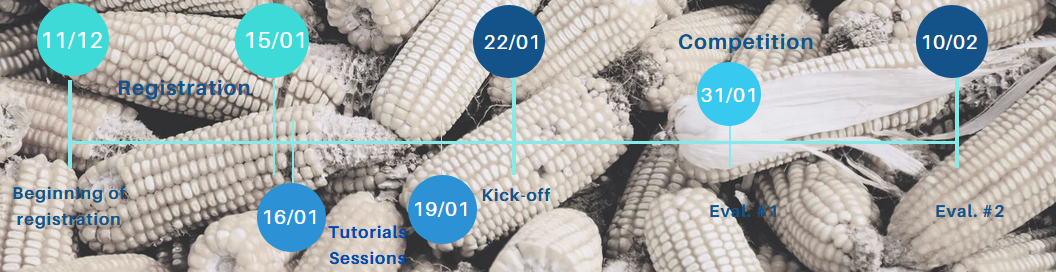
\includegraphics[width=\columnwidth]{figures/2024-Timeline_2.png}
            \caption{Chronologie officielle de GenHack 3 2024 \cite{polytechniqueGenhackHackathon}}
            \label{fig:ftcat}
        \end{figure}
        Dates clés:
        \begin{itemize}
            \item Inscription : Fermée le 15 janvier 2024.
            \item Sessions de tutorat et création d'équipes : 16-19 janvier 2024.
            \item Lancement : 22 janvier 2024.
            \item Compétition : 22 janvier - 10 février 2024.
            \item Évaluation n°1 : 3 février 2024.
            \item Évaluation n°2 : 10 février 2024.
        \end{itemize}
    \end{block}

    \begin{block}{Inscriptions et Règles de la Compétition}
        \textbf{Détails de l'inscription:}
        \begin{itemize}
            \item Inscriptions closes le 15 janvier 2024.
        \end{itemize}
        
        \textbf{Règles de la compétition:}
        \begin{itemize}
            \item Équipes de 3 à 5 étudiants.
            \item Code : Python seulement.
            \item Collaboration encouragée.
            \item Les membres de l'équipe gagnante doivent prouver leur statut d'étudiant.
        \end{itemize}
    
    \end{block}
\end{column}

    

   
    
\end{column}

\separatorcolumn
\end{columns}



\end{frame}
 \begin{block}{References}
    
        \AtNextBibliography{\small}
        \printbibliography
        
    \end{block}
\end{document}
